\subsection{Performance analysis of the algorithms}
\label{performance-analysys}
We said in~\ref{sort-fram} that sorting a data set is a computation described by a \textit{5-tuple} $\langle n$, $M$, $s$, $\Lambda$, $\sigma \rangle$, with $n$ the parallelism degree, $M$ the size of the data set, $s$ a seed for generating the data set, $\Lambda$ the algorithm and $\sigma$ a set of parameters depending on $\Lambda$. In reality, $\sigma$ is significative just for some algorithms; for instance, it can specify the \textit{stencil} (communication pattern) for the processes of a parallel algorithm or the value of ''\textit{K}'' in algorithms like \textit{K-way mergesort}. For each $\Lambda$, we will run single-shot computations (that is, there are not streams of data sets to sort) by varying $n$, $M$, $s$. Initially, $\sigma$ will be fixed for every computations. It is a convention that we will refer to \textit{small}, \textit{large} or \textit{huge} data sets for sizes that are respectively of the order of KBs, MBs and (at least) GBs. 

In order to analyze the performance of the algorithms from different perspective (e.g.: scalability of the specific algorithm, comparison of the time completion required by different algorithms to sort a specific data set and so on) we are going to show different types of graphics. Each graphic is defined by a 3-tuple $\langle x, y, plot \rangle $, where $x$ is the variable on the X axis, $y$ the variable on the Y axis and $plot$ a parameter that identifies a specific shape of that graphic. In particular, given $T$ the time completion of a computation, we will focus on the study of the following graphics:
\begin{itemize}
\item fixed $M$, a graphic $\langle n, T, \Lambda \rangle $ is necessary to see which is the best algorithm for sorting a data set of a certain size. 
\item fixed $\Lambda$, a graphic $\langle n, T, M \rangle$ is useful to see the scalability of $\Lambda$ by varying the computational grain. 
\item fixed $n$, a graphic $\langle \Lambda, T, M \rangle$ just for the sake  of curiosity to see, given a certain architecture with a fixed number of processors, which algorithm \textit{should} be used. (but not necessarily, due to the fact that architecture changes for a lot of factors) 
\end{itemize}

The parameters of the computations take the following values:
\begin{itemize}
\item $\Lambda \in \lbrace$Sequentialsort, Bitonicsort, Samplesort, Bucketsort, Mergesort, Quicksort, K-Way Mergesort, Load-Balanced Mergesort, Load-Balanced Multi-Way Mergesort$\rbrace$;
\item $n \in \lbrace$1, 2, 4, 8, 16, 32, 64, 128$\rbrace$; notice that the maximum value that $n$ can take depends on the specific architecture. 
\item $M \in \lbrace 2^{10 + i} : i = 0, ..., 25\rbrace$ elements (integers). So $M$ takes values from a few kilobytes to tens of gigabytes (recall that each integers is usually represented through 4 bytes).
\end{itemize} 

\subsubsection{Pianosa}
First, we will analyze the behavior of our algorithms for large data sets, then we will focus on huge data sets, finally on small data sets. 

\paragraph{Large data sets}
Figure~\ref{large-tc} shows the completion time for sorting large data sets. One thing is clearly visible: for parallelism degrees up to 8, sequential $qsort$ even outperforms almost all the algorithms; for parallelism degree 16 some algorithms improve a little the completion time ($Samplesort$, $Bucketsort$, $Mergesort$, $Load$-$Balanced$ $Multi$-$Way$ $Mergesort$), but anyway it keeps to be very close (same order magnitude) to the one of $qsort$. However, this result is not really surprising. Indeed, as we told in advance, we must take care of the following features:
\begin{itemize}
\item the computation performed on each element of the data set has fine grain;
\item the whole data set is of the order of MBs. In the best case, changing the parallelism degree from $2$ to $4$ (or at most from $4$ to $8$) and assuming a data set size of $400$ MB, we notice that almost all parallel algorithms significatively (but not ideally) improve the completion time. This is because each process can work on a portion of data that is still roughly a hundred of MBs. In all other cases, each process works on very smaller portion of data, so the parallelization, given that the computation on each element has fine grain, is not so useful. 
\item the cost and the number of communications that, as we saw in~\ref{test-env-pianosa}, may impact the completion time. We will further investigate and detail the impact of communications in the final version of the report.
\end{itemize}
These consideration aims at justifying the non-ideal scalability of the algorithms. We hope that for huge data sets we will be able to improve these results by increasing the time spent by each process on the sequential computation, hoping that it will be relatively larger than the one spent in communications. Surely, at least the difference between the time completion of parallel algorithms and the one of sequential qsort will become significant.
\begin{figure}[p]
	\centering
	\subfloat[Cost of sequential qsort.]{\label{large-sequential}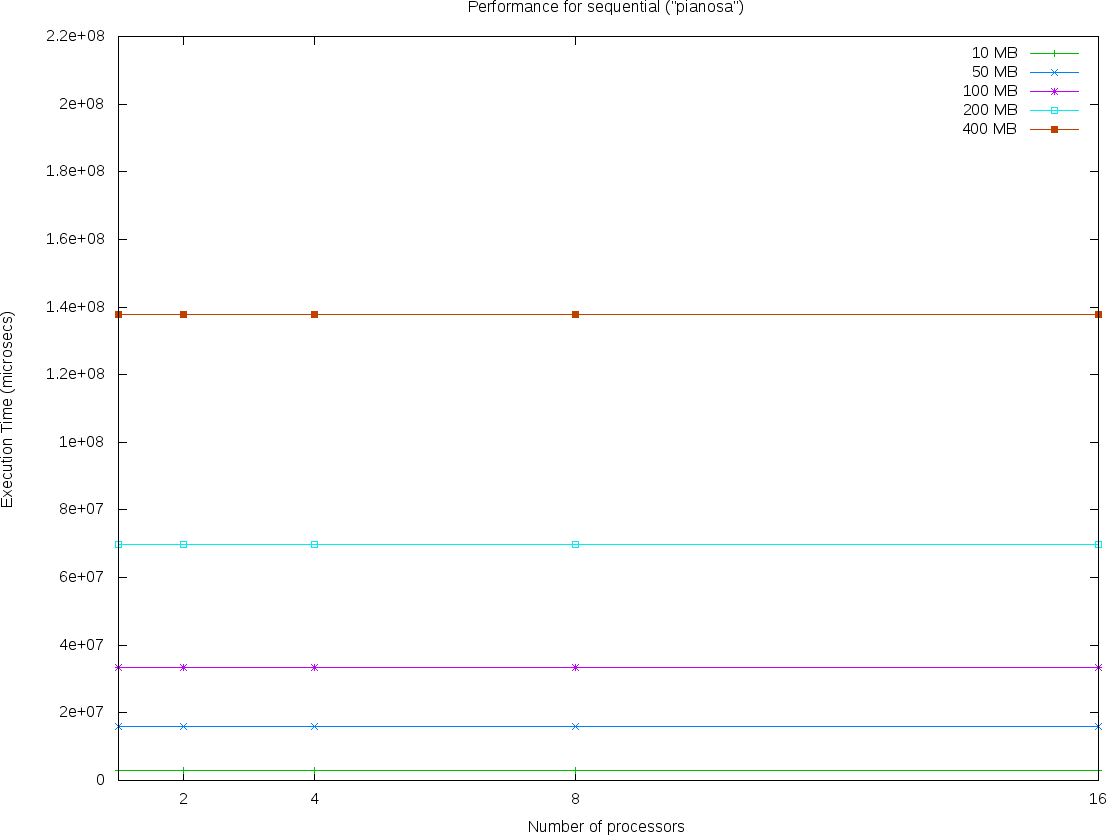
\includegraphics[width=0.4\textwidth]{results/large_sequential_pianosa}} 
	\hspace*{20pt}	
  	\subfloat[Bitonicsort.]{\label{large-bitonicsort}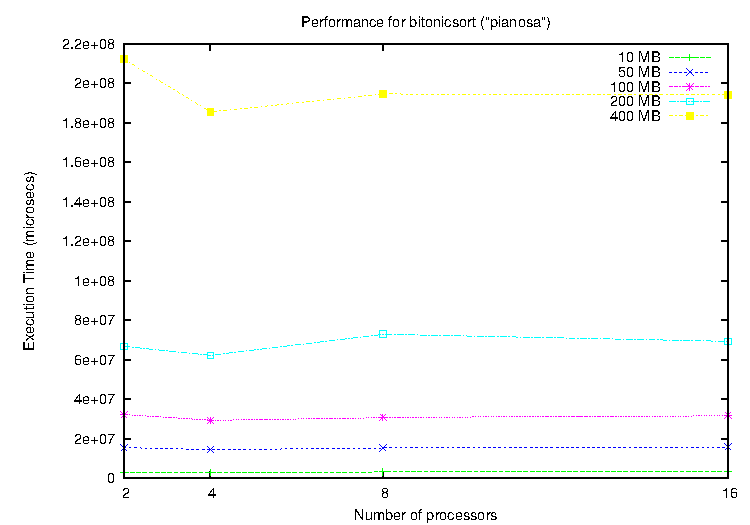
\includegraphics[width=0.4\textwidth]{results/large_bitonicsort_pianosa}}
  		
	\centering
	\subfloat[Bucketsort.]{\label{large-bucketsort}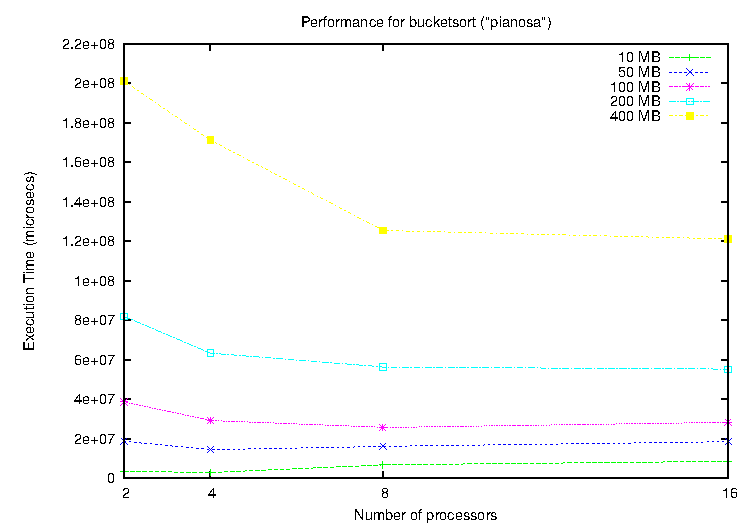
\includegraphics[width=0.4\textwidth]{results/large_bucketsort_pianosa}}  
  	\hspace*{20pt}
  	\subfloat[Samplesort.]{\label{large-samplesort}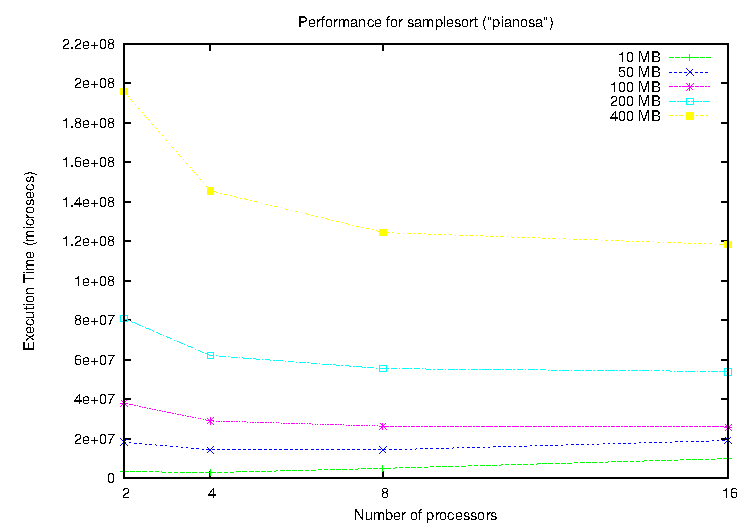
\includegraphics[width=0.4\textwidth]{results/large_samplesort_pianosa}}  
	
	\centering
  	\subfloat[Mergesort.]{\label{large-mergesort}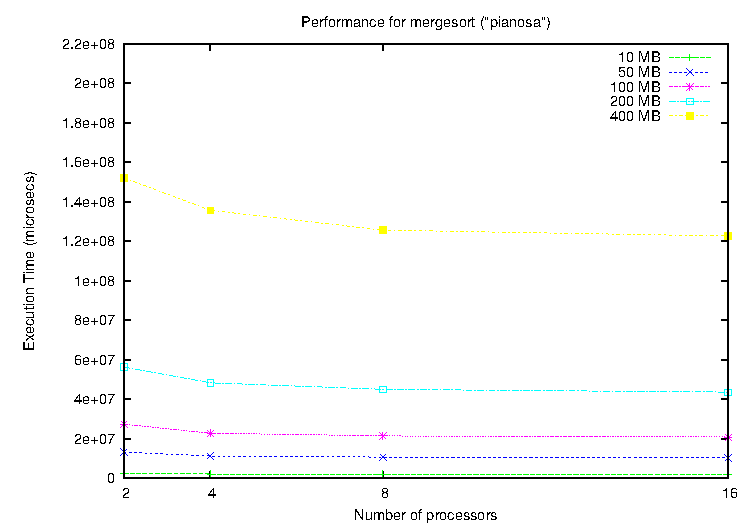
\includegraphics[width=0.4\textwidth]{results/large_mergesort_pianosa}}  
  	\hspace*{20pt}  
  	\subfloat[K-Way Mergesort.]{\label{large-kmerge}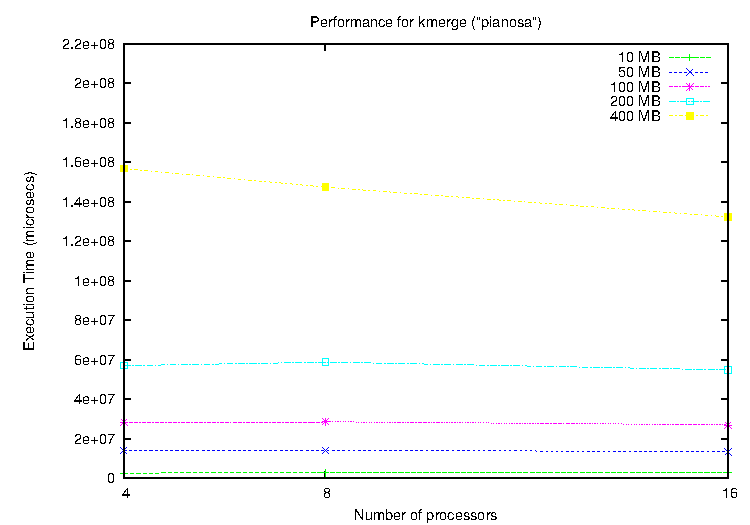
\includegraphics[width=0.4\textwidth]{results/large_kmerge_pianosa}} 
	
	\centering
  	\subfloat[Load-Balanced Mergesort.]{\label{large-lbmergesort}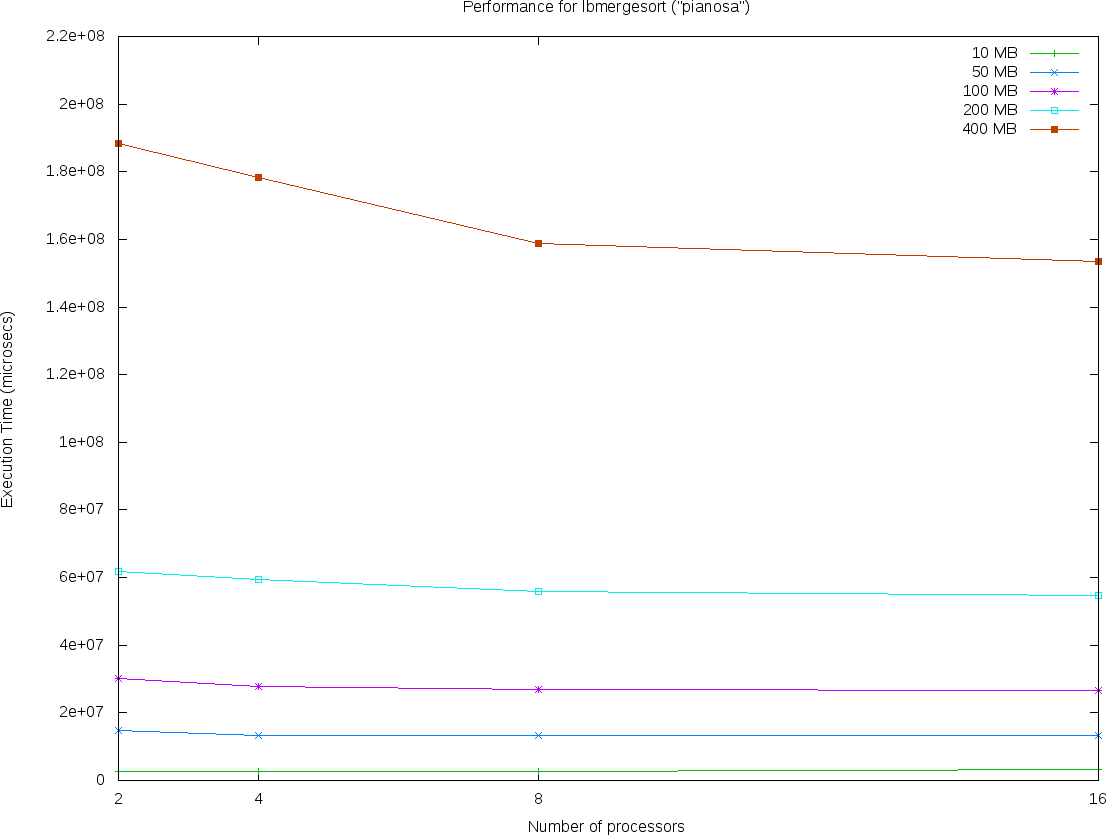
\includegraphics[width=0.4\textwidth]{results/large_lbmergesort_pianosa}}  
  	\hspace*{20pt}  
  	\subfloat[Load-Balanced Multi-Way Mergesort.]{\label{large-lbkmergesort}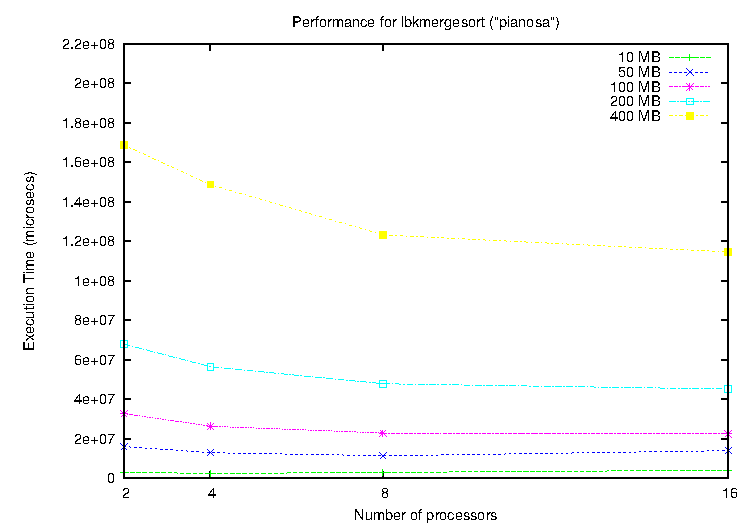
\includegraphics[width=0.4\textwidth]{results/large_lbkmergesort_pianosa}} 
  	
	\caption{Completion Time of the algorithms on Pianosa for large data sets.}
	\label{large-tc}
\end{figure}
 
\paragraph{Small data sets}
All our algorithms do not scale on Pianosa when the data set to sort is small (i.e. its size is of the order of hundreds of kilobytes); even worse, increasing the parallelism degree of the algorithm causes an increase of the completion time too. Figure~\ref{small-samplesort} shows the specific case of Samplesort; all other algorithms behave like Samplesort. This behavior is mainly due to the cost of communications between processes. If we model the cost of a $send$ as we did in~\ref{test-env} and if we look at the result obtained in~\ref{test-env-pianosa}, we can clearly see that the cost of sending a few kilobytes is of the order of milliseconds. On the other hand, the cost of sorting a small data set is of the order of milliseconds too (see Figure~\ref{small-sequential}; scale is not logarithmic to a better comparison with the other figures). These characteristics leads us to say, from a qualitative point of view, that the higher the parallelism degree, the higher both the number of communications and the overall time spent in sending data, so higher is even the overhead introduced by the parallelization. 

\begin{figure}[h]
	\centering
	\subfloat[Cost of sequential qsort.]{\label{small-sequential}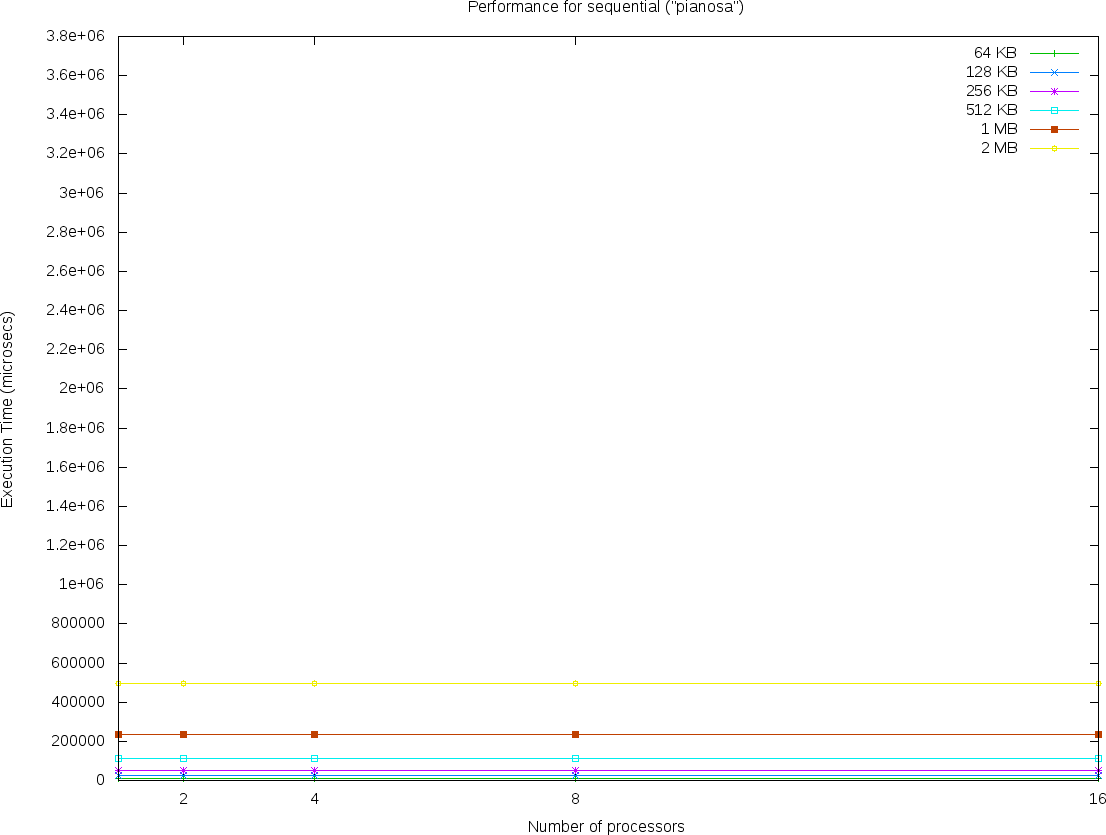
\includegraphics[width=0.4\textwidth]{results/small_sequential_pianosa}} 
	\hspace*{20pt}
  	\subfloat[Samplesort.]{\label{small-samplesort}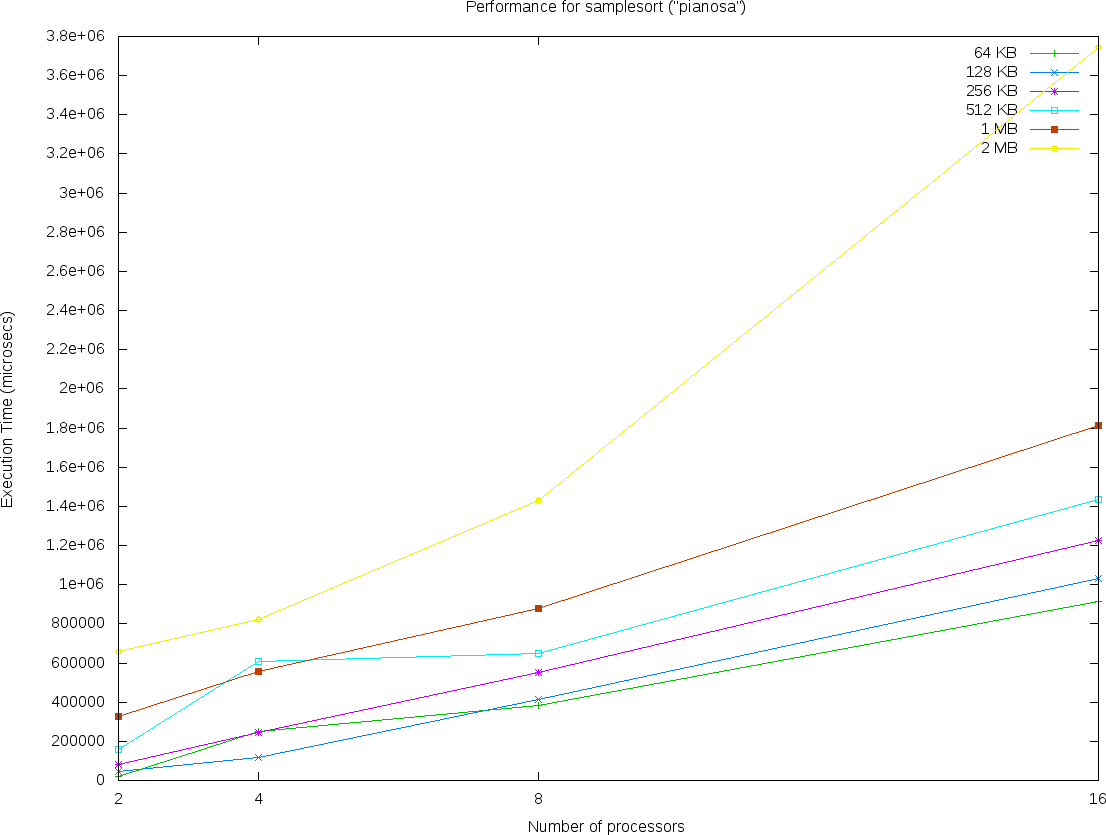
\includegraphics[width=0.4\textwidth]{results/small_samplesort_pianosa}}  
  	
  	\caption{Completion Time on Pianosa for small data sets.}
\end{figure}

\subsubsection{Physics}
